\subsection{Against the libraries}\label{sec:libraries}

A gap between a library default and a tuned structure measured inside one engine could be a property of that engine. Table~\ref{tab:libraries} times five libraries on \nLibraryCells{} cells (one scene at 1M, five at 25M, nine at 100M) under the sequential protocol of Section~\ref{sec:protocol}, each at its default and across its main parameter, next to our own defaults and the rule's pick, all relative to the cell's selected schema. Every library's answers were checked against the engine's query by query: no count differs anywhere, and the identifier sets differ only on $k$-nearest-neighbour queries whose $k$-th and $(k{+}1)$-th neighbours lie at the same single-precision distance, which the libraries break differently.

\begin{figure*}[tb]
\centering
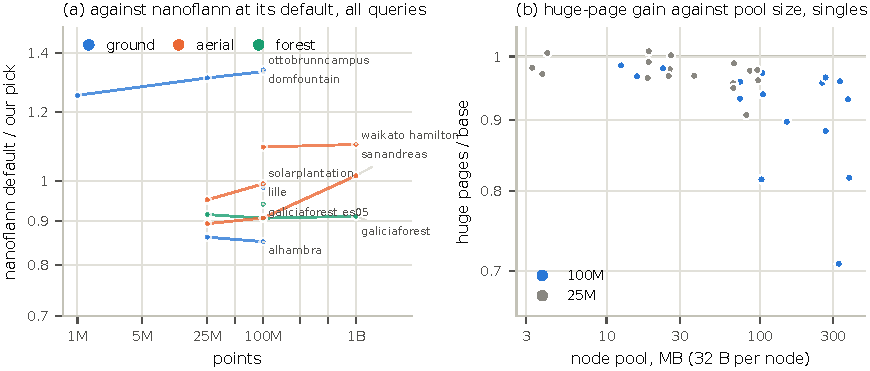
\includegraphics[width=\textwidth]{figures/fig_scale}
\caption{(a) nanoflann at its default leaf over the cell's selected schema, per scene and size, all queries of the trace, sequential protocol. (b) The huge-page arm over the base arm for every single structure of Section~\ref{sec:mechanism} against its node pool size: the gain grows with the pool, and the largest pools gain most.}
\label{fig:scale}
\end{figure*}

\begin{table}[t]
\centering\footnotesize
\caption{External libraries on the held-out traces, latency per query relative to the cell's selected schema (above 1: slower than our pick), geometric means over \nLibraryCells{} cells, for the trace's query mix and for its radius and $k$-nearest-neighbour queries separately; the last column is each library's own default over its best setting. Sequential protocol, median of three rotated rounds.}
\label{tab:libraries}
% generated by scripts/paper/tables.py; do not edit
\begin{tabular}{lrrrr}
\toprule
Library, setting & all & radius & kNN & own lever \\
\midrule
ours, octree default & 1.73 & 1.91 & 1.52 &  \\
ours, kd-tree default & 1.42 & 1.57 & 1.24 &  \\
ours, rule pick & 1.01 & 0.96 & 1.06 &  \\
nanoflann kd, def. & 1.02 & 1.27 & 0.72 & 1.07 \\
nanoflann kd, best & 0.95 & 1.18 & 0.68 &  \\
PCL KdTreeFLANN, def. & 2.59 & 3.51 & 1.58 &  \\
Open3D KDTreeFlann, def. & 1.60 & 2.13 & 1.00 &  \\
unibn octree, def. & -- & 1.65 & -- & 1.05 \\
unibn octree, best & -- & 1.56 & -- &  \\
Boost R-tree, def. & 2.46 & 2.32 & 2.50 & 1.04 \\
Boost R-tree, best & 2.37 & 2.24 & 2.40 &  \\
\bottomrule
\end{tabular}

\end{table}

\paragraph{nanoflann ties the tuned pick.} At its default leaf of ten points nanoflann~\cite{blanco2014nanoflann} is \nanoflannDefaultAll$\times$ our selected schema over the query mix, and at its best leaf of 16 to 32 it is \nanoflannBestAll$\times$: a tie at the default and a small win when tuned. The tie is made of two opposite differences. nanoflann is faster on every $k$-nearest-neighbour cell (\nanoflannDefaultKnn$\times$ at its default, \nanoflannBestKnn$\times$ at its best), because it updates the distance to a child cell along the split axis incrementally where our traversal recomputes a three-dimensional box distance per child. Our engine is faster on the radius queries of most cells (nanoflann at \nanoflannDefaultRadius$\times$ and \nanoflannBestRadius$\times$), because its leaves stream through reordered coordinate arrays where nanoflann gathers the original points through an index. Leaf for leaf, the two engines are at parity, and nanoflann's default is already the right structure for a three-dimensional scene: a sliding-midpoint kd-tree with a small leaf. Figure~\ref{fig:scale}a shows the ratio per scene and size: flat across the range measured here, with a slight drift in our favour as the cloud grows.

\paragraph{At a billion points.} The three clouds of the study that reach one billion points (a forest and two aerial surveys) were timed against nanoflann under the same sequential protocol, with a thousand replayed queries. The tie holds: nanoflann's default is \anchorNanoflannDefaultAll$\times$ the selected schema over the query mix (\anchorNanoflannDefaultMin{} to \anchorNanoflannDefaultMax{} across the three) and \anchorNanoflannBestAll$\times$ at its best leaf, ahead on the $k$-nearest-neighbour queries (\anchorNanoflannDefaultKnn$\times$) and behind on the radius queries (\anchorNanoflannDefaultRadius$\times$), as at every smaller size; it is ahead on the forest scan and behind on the two aerial ones, where the selected schema is a quadtree. Our own defaults are \anchorOursOctreeDefault{} and \anchorOursKdDefault$\times$ the pick there, the same gap as below. Nothing in the data suggests that either engine pulls away at a billion points.

\paragraph{The other libraries are slower by implementation.} The FLANN kd-tree of the Point Cloud Library is \pclKdAll$\times$ our pick, the Boost.Geometry R-tree \boostAll$\times$, Open3D's kd-tree \openThreeDAll$\times$, and the octree of Behley et al.\ \unibnRadius$\times$ on the radius queries it supports; the Point Cloud Library's octree search is \pclOctreeAll$\times$, and forty times off on the forest scans, where its voxels are either empty or overfull. Each library's own parameter recovers between \libraryLeverMin{} and \libraryLeverMax$\times$, so these gaps are not a matter of tuning: three implementations of the same kd-tree span a factor of 2.6 among themselves, which is the spread Elseberg et al.~\cite{elseberg2012comparison} found a decade ago. The structure a library implements and how it implements it both matter; the composition of structures does not appear in either.

\paragraph{What this does to the default gap.} Our own octree and median kd-tree defaults at leaf 32 are \oursOctreeDefaultOverPick$\times$ and \oursKdDefaultOverPick$\times$ the pick on these cells, and the rule's pick \ruleOverPick$\times$. The 1.6 to 1.7$\times$ gap of Section~\ref{sec:levers} is therefore the gap of a particular pair of defaults, an octree and a median-split kd-tree at a small leaf, and not of library defaults in general: a user of nanoflann already has the right structure for three-dimensional scenes, and a user of PCL or Open3D loses more to the implementation than to the structure. The claim the data supports is narrower and more useful than "defaults leave 1.7$\times$ on the table": choose a sliding-midpoint kd-tree for three-dimensional scenes and a quadtree for 2.5-dimensional ones, give it a leaf of 64 to 128 points, and then the implementation is what is left.
